\section{Metody iteracyjne}
%%%%%%%%%%%%%%%%
\begin{frame}{Metody iteracyjne $x = \phi(x)$}
	$f(x) = 0$ zapisujemy jako \fbox{$x = \phi(x)$} - $\infty$ liczbę sposobów:\linebreak
	
	Np:\linebreak
	$x + \ln(x) = 0 \rightarrow x = -\ln(x),\quad x = e^{-x},\quad \ldots$
	$x^{3} - 3x + 1 = 0 \rightarrow x = \frac{1}{3}(x^{3} + 1), x = \frac{1}{3 - x^{2}}, x = (1 - k) \cdot x + \frac{k}{3}(x^{3} + 1)$
	
	\begin{itemize}
		\item $x_{0}$ - początkowe przybliżenie pierwiastka $\alpha$
		\item generujemy ciąg $\left\{x_{i}\right\}$ stosując proces iteracyjny:
	\end{itemize}
	\[
		x_{i} = \phi(x_{i-1}),\quad i = 1, 2, \ldots \quad lub
		\begin{cases}
			y = \phi(x_{i-1})\\
			y = x_{i}
		\end{cases}
	\]
\end{frame}
%%%%%%%%%%%%%%%%
\begin{frame}{Metody iteracyjne $x = \phi(x)$}
	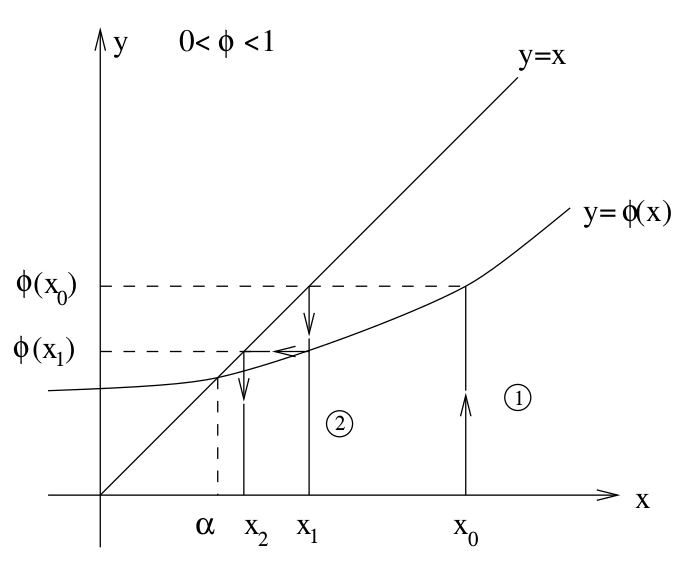
\includegraphics[width=.45\linewidth]{img/7/7_3_1}
	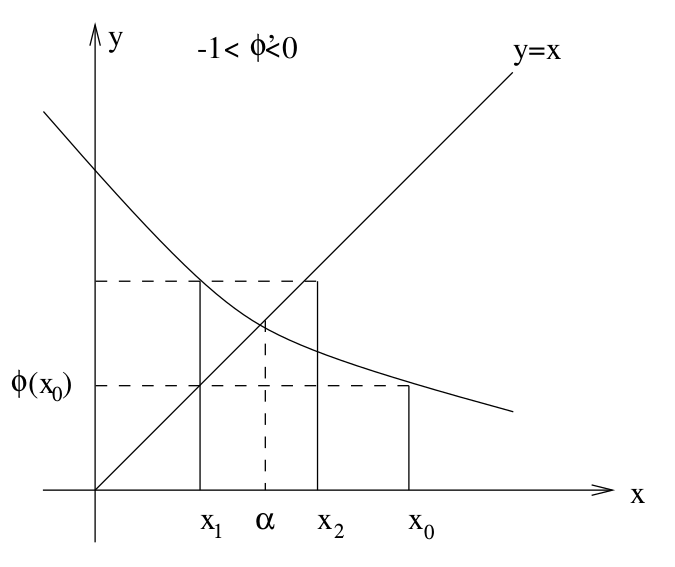
\includegraphics[width=.45\linewidth]{img/7/7_3_2}
\end{frame}
%%%%%%%%%%%%%%%%
\subsection{Twierdzenie o zbieżności procesu iteracyjnego}
\begin{frame}{Twierdzenie o zbieżności procesu iteracyjnego $x_{i+1} = \phi(x_{i})$}
	\begin{block}{Twierdzenie}
		\textbf{Niech:}
		\begin{enumerate}
			\item $x = \phi(x)$ ma pierwiastek $\alpha$
			\item na przedziale $I = \left[\alpha - a, \alpha + a\right]$ zachodzi $\lvert \phi'(x) \rvert \leq L < 1$, gdzie L jest stałą
		\end{enumerate}
		\vspace{0.5cm}
		\textbf{Wtedy: } dla dowolnego $x_{0} \in I$ :
		\begin{enumerate}
			\item $x_{i} \in I$, $i = 1, 2, \ldots$
			\item $\lim_{i \rightarrow \infty} x_{i} = \alpha$
			\item $\alpha$ jest jedynym pierwiastkiem $x = \phi(x)$ w $I$
		\end{enumerate}
	\end{block}
\end{frame}

\begin{frame}{Twierdzenie o zbieżności procesu iteracyjnego $x_{i+1} = \phi(x_{i})$}
	\textbf{Dowód:}
	\begin{enumerate}
		\item Niech $x_{i-1} \in I$
		\[
			x_{i} - \alpha = \phi(x_{i-1}) - \phi(\alpha) = (x_{i-1} - \alpha) \cdot \phi'(\eta_{i-1})
		\]
		z Tw. o wartości średniej; $\eta_{i-1} \in I$
		\[
			\lvert x_{i} - \alpha \rvert = \lvert x_{i-1} - \alpha \rvert \cdot \lvert \phi'(\eta_{i-1}) \rvert \leq \lvert x_{i-1} - \alpha \rvert \cdot L \qquad \Rightarrow x_{i} \in I \quad(*)
		\]
		
		\item $(*)$ używamy wielokrotnie
		\[
			\lvert x_{i} - \alpha \rvert \leq L \cdot \lvert x_{i-1} - \alpha \rvert \leq L^{2} \cdot \lvert x_{i-2} - \alpha \rvert \leq \ldots \leq L^{i} \cdot \lvert x_{0} - \alpha \rvert
		\]
		$L < 1$, $\lim_{i \rightarrow \infty} L^{i} = 0 \quad \Rightarrow \quad \lim_{i \rightarrow \infty} \lvert x_{i} - \alpha \rvert = 0$
	\end{enumerate}
\end{frame}
%%%%%%%%%%%%%%%
\begin{frame}{Twierdzenie o zbieżności procesu iteracyjnego $x_{i+1} = \phi(x_{i})$}
	\begin{enumerate}
		\setcounter{enumi}{2}
		\item Niech w $I$ oprócz pierwiastka $\alpha$ będzie pierwiastek $\beta$
		\[
			\alpha - \beta = \phi(\alpha) - \phi(\beta) = (\alpha - \beta) \cdot \phi'(\eta)
		\]
		\[
			\lvert \alpha - \beta \rvert = \lvert \alpha - \beta \rvert \cdot \underbrace{\lvert \phi'(\eta) \rvert}_{< 1} < \lvert \alpha - \beta \rvert \qquad \rightarrow \text{sprzeczność!}
		\]
		
		Zawsze: $x_{i-1} - \alpha = (x_{i} - \alpha) + (x_{i-1} - x_{i})$\linebreak
		Monotoniczna zbieżność\linebreak
		$\lvert x_{i-1} - \alpha \rvert \leq \lvert x_{i} - \alpha \rvert + \lvert x_{i-1} - x_{i} \rvert$ $\vert^{\cdot L + \text{fakt:}}_{\lvert x_{i} - \alpha \rvert \leq \lvert x_{i-1} - \alpha \rvert}$
		\[
			\lvert x_{i} - \alpha \rvert \leq \frac{L}{1 - L} \lvert x_{i-1} - x_{i} \rvert
		\]
		\[
			\frac{L}{1 - L} < 1 \text{ dla } L < \frac{1}{2}
		\]
	\end{enumerate}
\end{frame}
\subsection{Rząd zbieżności procedury iteracyjnej $x_{i} = \phi(x_{i-1})$}
%%%%%%%%%%%%%%
\begin{frame}{Rząd zbieżności procedury iteracyjnej $x_{i} = \phi(x_{i-1})$}
	\begin{enumerate}
		\item $\left\{x_{i}\right\} $ - zbieżność do $\alpha$
		\item ``szybkość'' zbieżności $\lvert \frac{\epsilon_{i}}{\epsilon_{i-1}} \rvert = $ ?
	\end{enumerate}
	\[
		\epsilon_{i} = x_{i} - \alpha = \phi(x_{i-1}) - \phi(\alpha)
	\]
	
	rozwinięcie względem $\alpha$
	\[
		\phi(x_{i-1}) = \sum_{j=0}^{p-1} \frac{1}{j!} \underbrace{(x_{i-1} - \alpha)^{j}}_{\epsilon_{i-1}} \cdot \phi^{(j)}(\alpha) + \frac{1}{p!}(x_{i-1}-\alpha)^{p} \cdot \phi^{(p)}(\eta_{i-1})
	\]
	
	$\eta_{i-1} \in (x_{i-1}, \alpha)$
	\[
		\epsilon_{i} = \sum_{j=1}^{p-1}\frac{1}{j!} \epsilon_{i-1}^{j} \cdot \phi^{(j)}(\alpha) + \frac{\epsilon_{i-1}^{p}}{p!} \phi^{(p)}(\eta_{i-1})
	\]
\end{frame}
%%%%%%%%%%%%%%%
\begin{frame}{Rząd zbieżności procedury iteracyjnej $x_{i} = \phi(x_{i-1})$}
	\textbf{Jeżeli: } $\phi'(\alpha) = \phi''(\alpha) = \ldots = \phi^{(p-1)}(\alpha) = 0,\quad \phi^{(p)}(\alpha) \neq 0$\linebreak
	
	\textbf{to: } $\epsilon_{i} = \frac{\epsilon_{i-1}^{p}}{p!} \phi^{(p)}(\eta_{i-1})$\linebreak
	
	$\lim_{i \rightarrow \infty} \lvert \frac{\epsilon_{i}}{\epsilon_{i-1}^{p}} \rvert = \frac{1}{p!} \lvert \phi^{(p)}(\alpha) \rvert$\linebreak
	
	$\lvert \frac{\epsilon_{i}}{\epsilon_{i-1}^{p}} \rvert$ - \textit{p-th order of convergence}\linebreak
	
	$\frac{1}{p!} \lvert \phi^{(p)}(\alpha) \rvert$ - asymptotic error constant
	\begin{tabbing}
		p = \= 1 - linear\\
		\> 2 - quadratic\\
		\> 3 - cubic
	\end{tabbing}
	
\end{frame}
%%%%%%%%%%%%%%
\begin{frame}{Rząd zbieżności procedury iteracyjnej $x_{i} = \phi(x_{i-1})$}
	Można konstruować metody iteracyjne $x_{i} = \phi(x_{i-1})$ dowolnego rzędu p - lecz: konieczne wyliczanie 0, 1, $\ldots$, $p-1$ pochodnych:\linebreak
	np. Richmod's:
	\[
	x_{i} = x_{i-1} - \frac{2 \cdot f(x_{i-1}) \cdot f'(x_{i-1})}{2 \cdot (f'(x_{i-1}))^{2} - f(x_{i-1}) f''(x_{i-1})}
	\]
\end{frame}